\section{Proces pomiarowy i~budowa zbioru danych}
\label{sec:measure}
Zgodnie z~opisem technik termowizyjnych przedstawionym w~sekcji
\ref{sec:thermovision}~zdecydowano się na przeprowadzenie pomiarów za pomocą
termowizji aktywnej.
Aby zrealizować pomiary przygotowano stanowisko laboratoryjne.
Kamera termowizyjna została umieszczona na statywie, a~do ogrzewania próbek
zdecydowano się wykorzystać lampę halogenową.

W~procesie termowizji aktywnej istotny jest charakter procesu nagrzewania
materiału.
Przy przygotowaniu pomiarów należy zdecydować pod jakim warunkiem zakończyć
przekazywanie ciepła do próbki.
Rozważono dwie możliwości:
\begin{enumerate}[a)]
    \item ogrzewanie próbek do osiągnięcia ustalonej temperatury,
    \item \label{it:heat_method}
          ogrzewanie próbek przez ustalony czas%
          \footnote{%
              Przy założeniu stałej masy ogrzewanych próbek.
          }.
\end{enumerate}
Zdecydowano się na metodę \ref{it:heat_method},~ze względu na wygodę jej
realizacji.
Doprowadzenie każdej próbki do tej samej temperatury wymaga pomiarów w~czasie
nagrzewania, co jest bardziej wymagające w~realizacji.
Wstępne obserwacje nagrań wskazują, że nagrzewanie materiału przez ustalony
czas, pozwala na obserwacje unikalnych wzorców stygnięcia ziaren.

Następnie wybrano czas nagrywania materiałów wideo.
Na podstawie próbnych nagrań zdecydowano się na ogrzewanie próbek przez jedną
minutę oraz rejestrację ich stygnięcia przez cztery minuty.
Taka konfiguracja daje, przy badanych próbkach rud miedzi, ostry i~szczegółowy
obraz w~początkowej fazie nagrywania oraz widocznie rozmazany i~mniej
kontrastowy obraz pod koniec stygnięcia.
Charakter procesu przejścia między tymi stanami pozwoli na klasyfikację badanych
ziaren rud miedzi.

Ostatnia decyzja kształtująca charakter pomiarów dotyczy chwili przechwytywania
stopklatek z~pozyskanych materiałów wideo.
Na podstawie obserwacji zdecydowano się eksportować pięć klatek, jedną na
początku każdej minuty nagrania.

Po ustaleniu planu eksperymentu pomiarowego przystąpiono do jego wykonania.
Zgodnie z~opisem badanych materiałów w~sekcji \ref{sec:grains},~zgromadzono
nagrania wideo dla czterech klas ziaren rud miedzi.
Ze względu na czasochłonność pomiarów dla każdej klasy materiału nagrano trzy
filmy.
Przy nagrywaniu stygnięcia tej samej klasy materiału pomiędzy pomiarami próbkę
poddawano przemieszaniu, aby uniknąć powtarzania struktur ułożenia ziaren.
Zgodnie z~opisem w~podsekcji \ref{subsec:camera_soft},~podczas zapisu zdjęć,
używano opcji automatycznego doboru zakresu temperatur.

Proces pomiarowy w~protypowych warunkach był obarczony brakiem dużej precyzji
i~powtarzalności.
Obserwacja uzyskanych nagrań pokazała, że obrazy tej samej klasy ziaren
niekoniecznie osiągały równą temperaturę po ogrzewaniu przez ustalony czas.
Problemem okazało się również dostosowanie ostrości obrazu z~kamery.
Jak wytłumaczono w~podsekcji \ref{subsec:lens}~wykorzystywana obiektyw cechuje
się bardzo małą głębią ostrości, co powoduje że drobne ruchy kamery mogą
spowodować utratę czytelności obrazu.
Z~kolei proces pomiarowy wymagał ciągłego przenoszenia próbki między
stanowiskiem do podgrzewania materiału oraz nagrywania filmów.
Należy mieć na uwadze że w~czasie układania próbek pod kamerą oraz poprawiania
ostrości postępowało stygnięcie ziaren, co sprzyjało brakowi powtarzalności
pomiarów.
Ze względu na przypadkowe utraty ostrości przy nagrywaniu oraz zbyt długi czas
przenoszenia i~przygotowania próbki do nagrywania, eksperyment wymagał czasem
powtarzania.
Ostatecznie jakość procesu pomiarowego oceniono na podstawie jego wyników
w~klasyfikacji ziaren, po skonstruowaniu sieci neuronowej.

\section{Analiza obrazów termowizyjnych}
Zgodnie z~planem pomiarów, przedstawionym w~sekcji \ref{sec:measure},~z~każdego
nagrania wybrano pięć stopklatek.
Podczas eksperymentu uzyskano łącznie dwanaście pomiarów, zawierających
sumarycznie 60~zdjęć.
W~ramach uczenia maszynowego jest to bardzo mały zbiór danych, biorąc jednak
pod uwagę wstępno-badawczy charakter pracy oraz czasochłonność procesu
pomiarowego zdecydowano, że jest to rozmiar zadawalający do pierwszych prób
klasyfikacji.
Zebrane materiały mają format JPEG.
Do oznaczania zdjęć przyjęto schemat nazw jak w~przykładzie: 115\_E11R\_1, gdzie
człony nazwy oznaczają kolejno: automatyczny numer nagrania w~programie FLIR
Tools, klasę próbki oraz minutę nagrania.

\subsection{Prezentacja przykładowej serii pomiarowej}
Jak opisano w rozdziale \ref{sec:measure}~jedna próbka w~zbiorze danych składa
się z~serii pięciu zdjęć o~malejącym kontraście i~szczegółowości.
Na rysunku \ref{fig:sample}~przedstawiono proces stygnięcia przykładowej
próbki 104~klasy E5R.
Wartości zakresu temperatur na zdjęciach maleją.
Wskazuje to na stopniowy spadek sumarycznej temperatury obserwowanego materiału.
Wraz z~upływem czasu obraz staje się także coraz mniej wyraźny i~kontrastowy.
Nagrzana próbka emituje ciepło ze swoich zróżnicowanych struktur w~niejednorodny
sposób.
Wraz z~ochłodzeniem ziaren temperatura na obrazie wyrównuje się i~kamera
termowizyjna rejestruje coraz mniej szczegółów.
Detale i~elementy charakterystyczne obrazu zlewają się na kolejnych zdjęciach.
Wraz z~opadaniem temperatury na zdjęciu pojawia się także coraz więcej szumów.
\begin{figure}[p]
    \hspace*{\fill}
    \begin{subfigure}{0.45\textwidth}
        \centering
        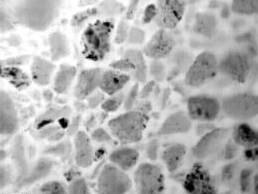
\includegraphics[width=\textwidth]{sample/104_E5R_0}
        \caption{Minuta: 0 \\
            Zakres temperatur: \SI{48.0}{\celsius} do
            \SI{53.0}{\celsius}}
    \end{subfigure}
    \hfill
    \begin{subfigure}{0.45\textwidth}
        \centering
        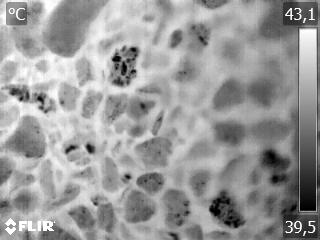
\includegraphics[width=\textwidth]{sample/104_E5R_1}
        \caption{Minuta: 1 \\
            Zakres temperatur: \SI{43.1}{\celsius} do
            \SI{39.5}{\celsius}}
    \end{subfigure}
    \hspace*{\fill}
    \vskip\baselineskip
    \hspace*{\fill}
    \begin{subfigure}{0.45\textwidth}
        \centering
        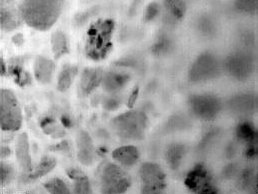
\includegraphics[width=\textwidth]{sample/104_E5R_2}
        \caption{Minuta: 2 \\
            Zakres temperatur: \SI{36.8}{\celsius} do
            \SI{39.5}{\celsius}}
    \end{subfigure}
    \hfill
    \begin{subfigure}{0.45\textwidth}
        \centering
        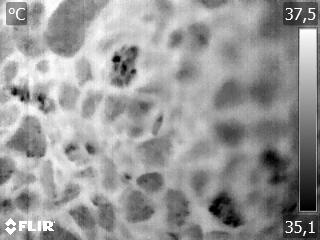
\includegraphics[width=\textwidth]{sample/104_E5R_3}
        \caption{Minuta: 3 \\
            Zakres temperatur: \SI{35.1}{\celsius} do
            \SI{37.5}{\celsius}}
    \end{subfigure}
    \hspace*{\fill}
    \vskip\baselineskip
    \hspace*{\fill}
    \begin{subfigure}{0.45\textwidth}
        \centering
        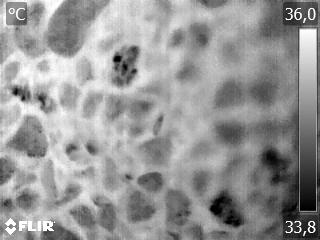
\includegraphics[width=\textwidth]{sample/104_E5R_4}
        \caption{Minuta: 4 \\
            Zakres temperatur: \SI{33.8}{\celsius} do
            \SI{36.8}{\celsius}}
    \end{subfigure}
    \hspace*{\fill}
    \caption{Zdjęcia procesu stygnięcia przykładowej próbki 104 klasy E5R}
    \label{fig:sample}
\end{figure}

\subsection{Przetwarzanie danych wizyjnych}
Wykorzystanie wizji komputerowej w~rozmaitych zadaniach często wymaga
odpowiedniego przygotowania używanych obrazów.
Do standardowych technik należą: wyrównywanie histogramu oraz redukcja szumów
i~wyostrzanie zdjęć.
Po analizie zebranych obrazów i~wypróbowaniu wymienionych technik zdecydowano
się jednak nie modyfikować zgromadzonych nagrań.
Użyty podczas pomiarów program \textsc{Flir} Tools posiada wbudowaną funkcję
doboru zakresu temperatur, co przekłada się na ekspozycję i~kontrast
eksportowanych zdjęć.
Próba wyrównywania histogramu oraz korekcji kontrastu sprawiłaby, że obraz
rozkładu temperatur na zdjęciu stałby się przekłamany.
Ze względu na niską, jak na standardy typowego przetwarzania zdjęć cyfrowych,
rozdzielczość obrazów zrezygnowano także z~redukcji szumów.
Wiele detali ziaren ma wielkość zaledwie paru pikseli, proces usuwania szumu
mógłby spowodować ich zanik.
Nie oznacza to jednak, że zdjęcia charakteryzują się przypadkową ekspozycją.
Algorytmy automatycznego doboru zakresu temperatur oprogramowania kamery
powodują, że jasność elementów na zdjęciu dobrze reprezentuje właściwości
cieplne obiektu.

\subsection{Odczyt zakresu pomiarowego temperatur z~obrazu}
Jak wspomniano w~sekcji \ref{subsec:camera_soft}~jednym z~kluczowych czynników
decydujących o~wyglądzie obrazów pochodzących z~kamery jest zakres temperatur
mapowany na kolory w~obrazie.
Niestety aplikacja \textsc{Flir} Tools nie pozwala na eksport zakresu temperatur
wraz ze zdjęciami w~formacie liczbowym.
W~czasie zapisu zdjęć oprogramowanie dodaje do nich interfejs z~aktywną skalą
pomiarową, jednak jest on graficznie naniesiony na obraz.
Aby ułatwić w~przyszłości pracę z~materiałami z~kamery opracowano mechanizm
ekstrakcji zakresu temperatur ze zdjęć pochodzących z~kamery.

W~celu odczytu wartości liczbowych z~obrazu posłużono się gotową siecią
neuronową zaprojektowaną do detekcji tekstu na zdjęciach.
Zdecydowano się na użycie popularnej biblioteki \emph{Pytesseract}%
\footnote{%
    Repozytorium projektu w~serwisie GitHub:
    \url{https://github.com/madmaze/pytesseract}
}.
Analizowane zdjęcia są kadrowane, by wyizolować odczytywane liczby.
Wycięte fragmenty mają bardzo małą rozdzielczość, aby ułatwić sieci
rozpoznawanie liczb, zdecydowano się przeskalować obrazy w~górę.
W~czasie skalowania włączono mechanizm anty aliasingu aby wyrównać krawędzie
cyfr.
Ponieważ używana sieć uznaje za tło kolor biały oraz poszukuje liczb w~kolorze
czarnym, barwy na zdjęciu odwrócono.
Następnie obraz poddano binaryzacji metodą \emph{otsu}.
Jest to popularna i~wydajna metoda binaryzacji, jej efektywność jest maksymalna
kiedy liczba pikseli tła oraz pierwszego planu jest zbliżona
\cite{sezgin_thresholding}.
Z~tego powodu poprawne kadrowanie liczb sprzyja jakości ich binaryzacji.
Na rysunku \ref{fig:temp_bounds}~przedstawiono kolejne etapy przygotowania
obrazu do rozpoznania liczb.
Implementację opisanego mechanizmu odczytywania zakresu temperatur ze zdjęć
przedstawiono na listingu \ref{lst:temp_bounds}.
\begin{figure}[htbp]
    \hspace*{\fill}
    \begin{subfigure}{0.45\textwidth}
        \centering
        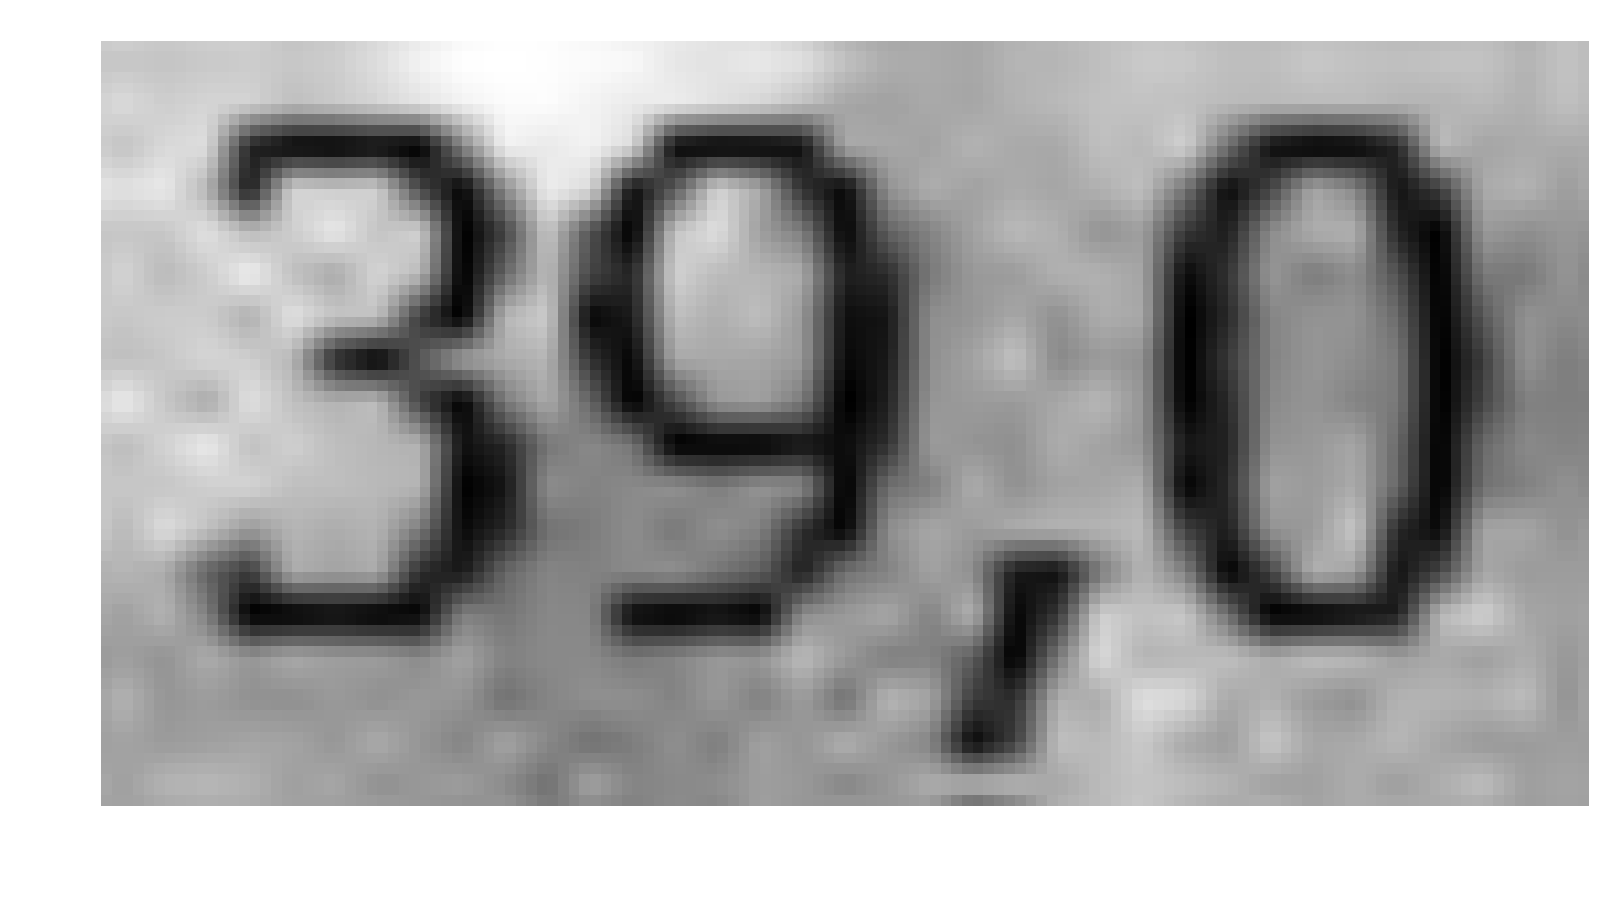
\includegraphics[width=\textwidth]{temp_bounds_scale}
        \caption{Przeskalowany kadr z~liczbą}
        \label{fig:temp_bounds_scale}
    \end{subfigure}
    \hfill
    \begin{subfigure}{0.45\textwidth}
        \centering
        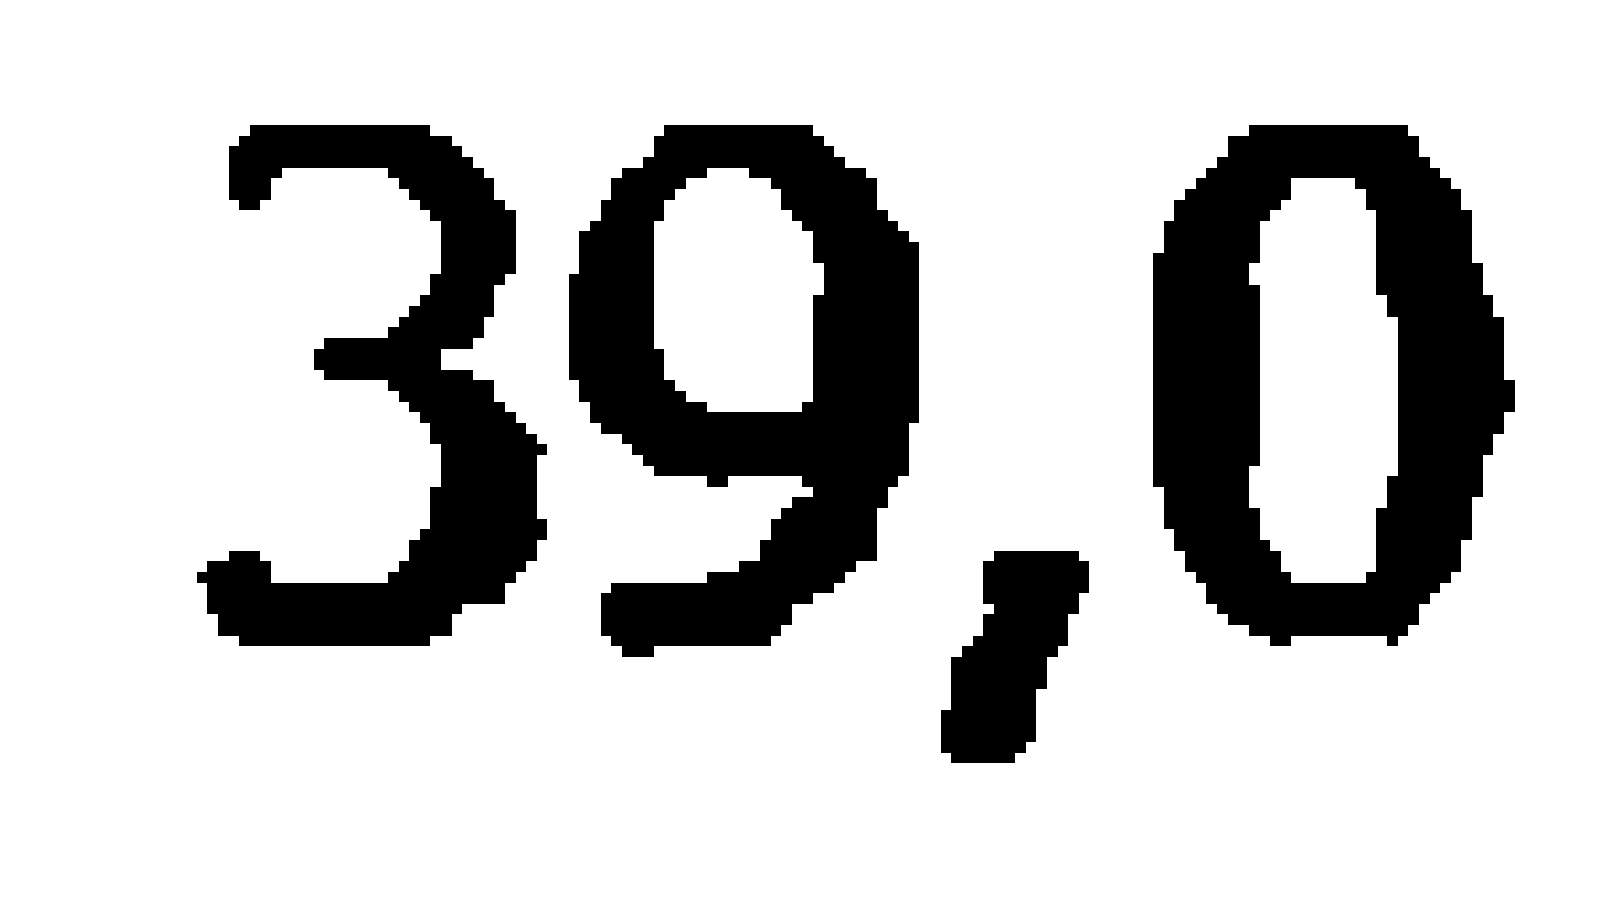
\includegraphics[width=\textwidth]{temp_bounds_bin}
        \caption{Kadr z~liczbą po binaryzacji}
        \label{fig:temp_bounds_bin}
    \end{subfigure}
    \hspace*{\fill}
    \caption{Przygotowanie zakresu temperatur do odczytu przez sieć neuronową}
    \label{fig:temp_bounds}
\end{figure}
\begin{listing}[htbp]
\begin{minted}{python}
def get_temperature_bounds(img, bounds=(((6, 24), (283, 318)),
                                        ((219, 236), (283, 318)))):
    '''Extract temperature values from FLIR UI on image.'''
    img = invert(img)
    temp_txt = []
    for bound in bounds:
        bound_img = img[slice(*bound[0]), slice(*bound[1])]
        bound_img = rescale(bound_img, 4, anti_aliasing=True)
        thr = threshold_otsu(bound_img)
        img_txt = bound_img > thr
        img_txt = Image.fromarray(img_txt)
        temp = pytesseract.image_to_string(img_txt, config='digits')
        if temp != '':
            temp = float(temp) / 10
        else:
            temp = 0
        temp_txt.append(temp)
    return temp_txt
\end{minted}
\caption{Funkcja języka Python odczytująca zakres temperatur ze zdjęć}
\label{lst:temp_bounds}
\end{listing}

\section{Eksploracja danych}
Aby móc klasyfikować dane należy zastanowić się nad cechami, którymi się różnią.
Na rysunku \ref{fig:sample_compare}~przedstawiono porównanie stygnięcia dwóch
rodzajów próbek: E5R oraz E6R.
W~klasyfikacji użyteczne będą dane, które są unikalne dla danej klasy.
Posiadane dane stanowią serie obrazów postępującego procesu studzenia materiału.
Aby dobrze wykorzystać zebrane zdjęcia należy szukać cech charakterystycznych
w~całym procesie stygnięcia.
\begin{figure}[htbp]
    \hspace*{\fill}
    \begin{subfigure}{0.3\textwidth}
        \centering
        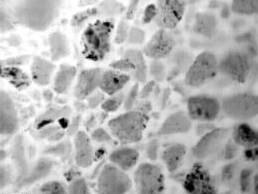
\includegraphics[width=\textwidth]{sample/104_E5R_0}
        \caption{Próbka 104\_E5R\_0}
    \end{subfigure}
    \hfill
    \begin{subfigure}{0.3\textwidth}
        \centering
        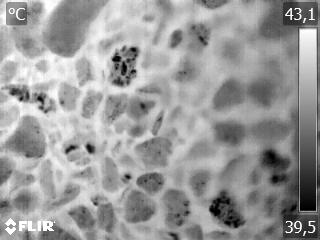
\includegraphics[width=\textwidth]{sample/104_E5R_1}
        \caption{Próbka 104\_E5R\_1}
    \end{subfigure}
    \hfill
    \begin{subfigure}{0.3\textwidth}
        \centering
        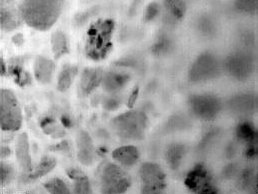
\includegraphics[width=\textwidth]{sample/104_E5R_2}
        \caption{Próbka 104\_E5R\_2}
    \end{subfigure}
    \hspace*{\fill}
    \vskip\baselineskip
    \hspace*{\fill}
    \begin{subfigure}{0.3\textwidth}
        \centering
        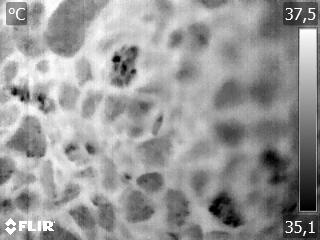
\includegraphics[width=\textwidth]{sample/104_E5R_3}
        \caption{Próbka 104\_E5R\_3}
    \end{subfigure}
    \hfill
    \begin{subfigure}{0.3\textwidth}
        \centering
        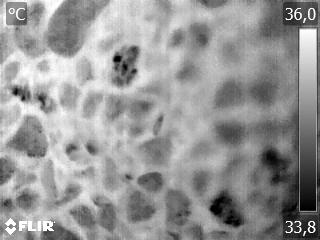
\includegraphics[width=\textwidth]{sample/104_E5R_4}
        \caption{Próbka 104\_E5R\_4}
    \end{subfigure}
    \hfill
    \begin{subfigure}{0.3\textwidth}
        \centering
        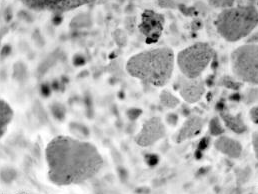
\includegraphics[width=\textwidth]{sample/117_E6R_0}
        \caption{Próbka 117\_E6R\_0}
    \end{subfigure}
    \hspace*{\fill}
    \vskip\baselineskip
    \hspace*{\fill}
    \begin{subfigure}{0.3\textwidth}
        \centering
        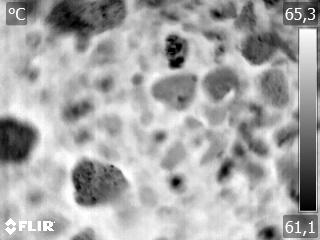
\includegraphics[width=\textwidth]{sample/117_E6R_1}
        \caption{Próbka 117\_E6R\_1}
    \end{subfigure}
    \hfill
    \begin{subfigure}{0.3\textwidth}
        \centering
        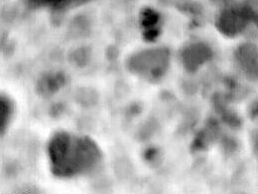
\includegraphics[width=\textwidth]{sample/117_E6R_2}
        \caption{Próbka 117\_E6R\_2}
    \end{subfigure}
    \hfill
    \begin{subfigure}{0.3\textwidth}
        \centering
        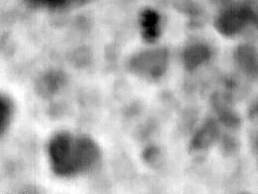
\includegraphics[width=\textwidth]{sample/117_E6R_3}
        \caption{Próbka 117\_E6R\_3}
    \end{subfigure}
    \hspace*{\fill}
    \vskip\baselineskip
    \hspace*{\fill}
    \begin{subfigure}{0.3\textwidth}
        \centering
        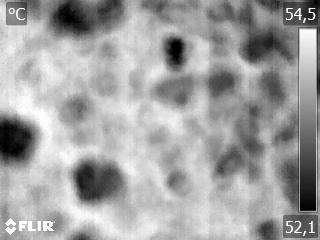
\includegraphics[width=\textwidth]{sample/117_E6R_4}
        \caption{Próbka 117\_E6R\_4}
    \end{subfigure}
    \hspace*{\fill}
    \caption{Porównanie procesu stygnięcia próbek klasy E5R oraz E6R}
    \label{fig:sample_compare}
\end{figure}

\subsection{Wybór cech obrazu użytecznych w~klasyfikacji}
\label{subsec:feature_extraction}
Po przyjrzeniu się rysunkowi \ref{fig:sample_compare}~widoczne jest, że w~próbce
E6R temperatura ziaren zaczęła wyrównywać się szybciej.
Zdjęcia tej próbki wcześniej stają się szare i~tracą kontrast.
Na podstawie analizy nagrań rozpatrzono następujące możliwości ekstrakcji ich
cech charakterystycznych:
\begin{enumerate}[a)]
    \item \label{it:cnn}
          klasyfikacja całych zdjęć z~użyciem zaawansowanych sieci
          konwolucyjnych,
    \item \label{it:fft}
          analiza częstotliwościowa obrazów,
    \item \label{it:glcm}
          użycie macierzy \textsc{glcm},
    \item \label{it:edge}
          detekcja krawędzi ziaren i~wyznaczanie reprezentacji liczbowej
          ich kształtów,
    \item \label{it:blob}
          śledzenie zlewania się i~zanikania małych detali na obrazie.
\end{enumerate}
Wszystkie przedstawione opcje mają uzasadnienie i~mogą się dobrze sprawdzić jako
podstawa klasyfikacji.
Metody \ref{it:fft},~\ref{it:glcm}~oraz \ref{it:edge}~były już w~różnym stopniu
badane w~ramach działaności Politechniki Śląskiej \cite{budzan_grains}.
Należy rozpatrzeć, którą technikę wykorzystać do budowy prototypu klasyfikatora.

Metoda bazująca na sieciach konwolucyjnych może wykorzystywać najnowsze
rozwiązania w~dziecinie uczenia maszynowego.
Utrudnieniem w~użyciu tej metody jest bardzo mały rozmiar posiadanego zbioru
danych.
Na zgromadzonych obrazach znajdują się zarówno użyteczne informacje, jak i szumy
pomiarowe, a~złożoność jednego zdjęcia jest na tę chwilę nieproporcjonalna do
wielkości zestawu danych.
Pomysł ten można wypróbować po rozszerzeniu zbioru nagrań.

Technika polegająca na analizie częstotliwościowej obrazów wymaga zastosowania
transformacji Fouriera.
Takie podejście charakteryzuje się złożonością obliczeniową.
Dodatkowo efekt analizy widmowej może być nieoczywisty w~interpretacji.
Wynikiem zastosowania transformacji Fouriera na obrazach są dwuwymiarowe
macierze.
Użycie takich danych wejściowych może wymagać konstrukcji złożonych sieci
neuronowych.
Analizę widmową ziaren przeprowadzono w~pracach naukowców Politechniki Śląskiej,
w~rozpatrywanym przypadku zdecydowano się na poszukiwanie innego rozwiązania.

Macierz \textsc{glcm} (ang. \textit{Gray-Level Co-Occurrence Matrix}), 
na której może bazować opcja \ref{it:glcm},~to tablica zawierająca informacje
o~relacjach wszystkich par pikseli w~obrazie.
Pozwala ona na analizę takich wartości jak: kontrast, korelacja, energia oraz
homogeniczność.
Jest to opcja dająca możliwość analizy dużej ilości informacji, z~pewnością
warta rozpatrzenia, jednak dosyć skomplikowana.
Zdecydowano się na wybór mniej złożonej metody.

W~obrazie można także wykrywać kształty ziaren za pomocą filtrów detekcji
krawędzi.
Opcję tę testowano przy pomocy filtra \emph{Canny}.
Uzyskane krawędzie nie pozwalają jednak na łatwą detekcję kształtów.
Tradycyjna segmentacja ziaren jest trudna ze względu na małą rodzielczość oraz
duże upakowanie ziaren.
Operacje morfologiczne domykania kształtów powodowały bardzo duże zmiany
w~obrazie i~zlewały ziarna.
Rozwój takiego podejścia przy analizowanych obrazach wymaga zaawansowanej
i~ostrożnej obróbki zdjęć.

Ostatnia opcja \ref{it:blob}~wynika z~obserwacji detali na obrazach.
Na przedstawionych zdjęciach próbek można zauważyć drobne ciemne punkty, które
są obszarami o~wolniejszej wymianie ciepła z~otoczeniem niż reszta powierzchni
ziaren.
Jest to spowodowane ich niską emisyjnością cieplną.
Na rysunku \ref{fig:blob_detail}~przedstawiono zbliżenie na grupę takich detali,
w~czterech częściach procesu stygnięcia.
\begin{figure}[h]
    \hspace*{\fill}
    \begin{subfigure}{0.3\textwidth}
        \centering
        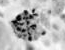
\includegraphics[width=\textwidth]{sample/detail_119_E5R_0}
        \caption{Grupa detali w~próbce 119\_E5R\_0}
    \end{subfigure}
    \hfill
    \centering
    \begin{subfigure}{0.3\textwidth}
        \centering
        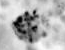
\includegraphics[width=\textwidth]{sample/detail_119_E5R_1}
        \caption{Grupa detali w~próbce 119\_E5R\_1}
    \end{subfigure}
    \hfill
    \begin{subfigure}{0.3\textwidth}
        \centering
        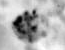
\includegraphics[width=\textwidth]{sample/detail_119_E5R_2}
        \caption{Grupa detali w~próbce 119\_E5R\_2}
    \end{subfigure}
    \hspace*{\fill}
    \caption{Zbliżenie na charakterystyczne grupy detali materiału}
    \label{fig:blob_detail}
\end{figure}

Analizując próbki można zauważyć, że wraz ze stygnięciem, ciemne punkty
w~grupach zlewają się, a~następnie zanikają.
Dodatkowo ich liczba dla poszczególnych klas materiałów jest różna.
Zdecydowano się na wybór metody polegającej na śledzeniu liczby tych punktów
i~ich zaniku.
Taka analiza wiąże się z~przetwarzaniem obrazów i~utworzeniem algorytmów
śledzenia detali.
Opcja ta jest obiecująca, ponieważ nawet podczas wstępnej obserwacji próbek
można dopatrywać się zależności miedzy klasami, a~obecnością omawianych detali.
Można również zaobserwować, że w~czasie stygnięcia na kolejnych zdjęciach
pojawiają się sporadycznie także nowe detale.
Przy zdecydowanej tendencji do zanika i~rozmywania plam zjawisko ich powstawania
jest jednak pomijalne.
Fakt pojawiania się nowych detali wzięto pod uwagę przy późniejszym procesie
projektowania algorytmów ich śledzenia.

\subsection{Wybór algorytmu detekcji ziaren}
\label{subsec:blob_detect}
Zgodnie z~rozważaniami przedstawionymi w~podsekcji
\ref{subsec:feature_extraction}~%
w~celu klasyfikacji ziaren zdecydowano się na obserwację ilości puntów o~małej
emisyjności
Należy więc wybrać metodę detekcji charakterystycznych elementów.
W~wykrywaniu omawianych detali użyteczne są algorytmy wykrywania plam na
podstawie analizy pochodnych wartości w~obrazie.
Biblioteka Scikit-image udostępnia trzy algorytmy tego typu wykorzystujące:
\begin{enumerate}[a)]
    \item laplasjan funkcji Gaussa,
    \item różnicę funkcji Gaussa,
    \item wyznacznik Hesjanu.
\end{enumerate}
Przedstawione algorytmy pozwalają na wykrycie na obrazie plam o~kształcie
zbliżonym do kolistego oraz oszacowanie ich promieni.
Badane detale, przedstawione na rysunku \ref{fig:blob_detail},~mają kształt
zbliżony do kolistego, więc próba użycia rozpatrywanych algorytmów jest
uzasadniona.
Należy porównać dostępne warianty detekcji i~wybrać algorytm, który działa
najskuteczniej na zgromadzonych próbkach.

Metoda bazująca na laplasjanie funkcji Gaussa jest najdokładniejsza, ale także
najwolniejsza.
Funkcja Gaussa, jest dana wzorem \ref{eq:gaussian}.
\begin{equation}
    P(x) = \frac{1}{{\sigma \sqrt {2\pi } }}
    e^{{{ - \left( {x - \mu } \right)^2 }
    \mathord{\left/ {\vphantom {{ - \left( {x - \mu } \right)^2 }
            {2\sigma ^2 }}} \right. \kern-\nulldelimiterspace} {2\sigma ^2 }}}
    \label{eq:gaussian}
\end{equation}
\begin{samepage}%
Symbole we wzorze mają następujące znaczenia:
\begin{description}
    \item[$ \sigma $] to odchylenie standardowe,
    \item[$ \mu $] to wartość średnia.
\end{description}
\end{samepage}
Laplasjan to operator różniczkowy drugiego rzędu.
Omawiany algorytm oblicza wartości funkcji Gaussa dla coraz większego odchylenia
standardowego i~układa je w~sześcianie.
Poszukiwane plamy to lokalne maksima w~tym sześcianie.
Wadą tego rozwiązania jest bardzo wolne wykrywanie dużych plam z~powodu
złożoności obliczeniowej.

Różnica funkcji Gaussa jest metodą podobną do poprzedniej.
Ponownie rozmywa ona obrazy z~narastającymi odchyleniami standardowymi z~użyciem
funkcji Gaussa.
Następnie różnice rozmytych obrazów są układane w~sześcianie, gdzie maksima to
plamy.
Metoda ta jest szybsza i~mniej dokładna od algorytmu bazującego na laplasjanie
funkcji Gaussa, ale podobnie jak ona jest wolna w wykrywaniu dużych elementów.

Ostatnia metoda jest najszybsza, ale najmniej dokładna.
Polega na wyszukiwaniu maksimów w~macierzy Hesjanu.
Jest to macierz drugich pochodnych cząstkowych.
Postać takiej macierzy w~n-wymiarowej przestrzeni zmiennych $ x $ przedstawia
wzór \ref{eq:hessian}.~%
Prędkość tej metody nie zależy od wielkości wykrywanych plam, ale małe elementy
mogą nie zostać przez nią wykryte \cite{scikit_reference}.
\begin{equation}
    H = \begin{bmatrix}
        \dfrac{\partial^2 f}{\partial x_1^2} &
        \dfrac{\partial^2 f}{\partial x_1\,\partial x_2} &
        \cdots & \dfrac{\partial^2 f}{\partial x_1\,\partial x_n} \\[2.2ex]
        \dfrac{\partial^2 f}{\partial x_2\,\partial x_1} &
        \dfrac{\partial^2 f}{\partial x_2^2} &
        \cdots & \dfrac{\partial^2 f}{\partial x_2\,\partial x_n} \\[2.2ex]
        \vdots & \vdots & \ddots & \vdots \\[2.2ex]
        \dfrac{\partial^2 f}{\partial x_n\,\partial x_1} &
        \dfrac{\partial^2 f}{\partial x_n\,\partial x_2} &
        \cdots &
        \dfrac{\partial^2 f}{\partial x_n^2}
    \end{bmatrix}
    \label{eq:hessian}
\end{equation}

Porównanie działania wymienionych metod przedstawiono na grafice
\ref{fig:blob_compare}.~%
Zgodnie z~teoretycznym opisem funkcji najlepsza okazała się metoda Laplasjanu
funkcji Gaussa.
Funkcję korzystającą z~wyznacznika Hesjanu należy odrzucić, ponieważ
w~rozważanym przypadku istotne jest wykrywanie małych plam.
Z~tego samego powodu korzystne jest użycie najdokładniejszej funkcji.
Ponieważ program nie powinien wykrywać dużych elementów, nie ma ryzyka zbyt
powolnych obliczeń na obszernych plamach.
\begin{figure}[h]
    \hspace*{\fill}
    \begin{subfigure}[t]{0.3\textwidth}
        \centering
        \input{figures/blob_detection_compare_LoG}
        \caption{Laplasjan funkcji Gaussa}
    \end{subfigure}
    \hfill
    \begin{subfigure}[t]{0.3\textwidth}
        \centering
        \input{figures/blob_detection_compare_DoG}
        \caption{Różnica funkcji Gaussa}
    \end{subfigure}
    \hfill
    \begin{subfigure}[t]{0.3\textwidth}
        \centering
        \input{figures/blob_detection_compare_DoH}
        \caption{Wyznacznik Hesjanu}
    \end{subfigure}
    \hspace*{\fill}
    \caption{Porównanie bibliotecznych algorytmów wykrywania plam na obrazie}
    \label{fig:blob_compare}
\end{figure}

Aby wybrana funkcja laplasjanu funkcji Gaussa wykrywała tylko małe plamy należy
podać jej odpowiednie parametry.
Uczyniono to już na etapie porównania metod detekcji.
Wywołanie omawianej funkcji ma postać przedstawioną na listingu
\ref{lst:find_blobs}.~%
Funkcji podano dwa dodatkowe argumenty, które są istotne dla pożądanego
działania.
Argument \mintinline{python}{max_sigma} ogranicza odchylenie standardowe
obliczanych funkcji Gaussa, przez co wykrywane są tylko małe elementy.
Drugi argument \mintinline{python}{threshold} decyduje o~poziomie, powyżej
którego punkt jest uznany za maksimum w~sześcianie laplasjanów.
Domyślna wartość tego argumentu \mintinline{python}{threshold} okazała się zbyt
duża, zmniejszono ją aby wykrywać bardziej subtelne detale.
Na podstawie opisanego wywołania metody laplasjanu funkcji Gaussa opracowano
funkcję zwracającą położenie i~promienie wykrytych plam.
\begin{listing}[htb]
\begin{minted}{python}
def find_blobs(img):
    '''
    Find blobs in given image and get list of their positions
    and radiuses.
    '''
    # Detect blobs with Difference of Gaussian
    blobs = blob_dog(img, max_sigma=2, threshold=0.1)
    # Get blobs radiuses from each kernel sigma
    blobs[:, 2] = blobs[:, 2] * sqrt(2)
    return blobs
\end{minted}
\caption{Funkcja języka Python wykrywająca detale na obrazie}
\label{lst:find_blobs}
\end{listing}

\subsection{Algorytm śledzenia ziaren w~serii zdjęć}
\label{subsec:blob_tracking}
Użycie funkcji bibliotecznych opisanych w~podsekcji \ref{subsec:blob_detect}~%
pozwala na detekcję detali na pojedynczym zdjęciu.
Aby wykorzystać detekcję plam w~serii pięciu zdjęć, które reprezentują
stygnięcie jednej próbki, należy opracować zestaw funkcji śledzący zmiany na
obrazie.
Na tym etapie prac nie jest jednoznaczne jaki sposób obserwacji i~zliczania
detali będzie najlepszy do późniejszego prototypowania sieci neuronowej
klasyfikującej ziarna rud miedzi.
Dlatego zdecydowano się na napisanie funkcji zliczania plam, tak by umożliwić
trzy warianty pracy algorytmu:
\begin{enumerate}[a)]
    \item \label{it:all_blob}
          zliczanie wszystkich detali na każdym etapie stygnięcia,
    \item \label{it:remaining_blob}
          zliczanie detali śledzonych od początku stygnięcia,
    \item \label{it:ratio_blob}
          zliczanie stosunku śledzonych detali do ich ilości na początku
          stygięcia.
\end{enumerate}
Przez śledzenie detali rozumiane jest zliczanie jedynie tych plam, które były
wykryte na początku stygnięcia.
Oznacza to, że metody \ref{it:remaining_blob}~oraz \ref{it:ratio_blob}~ignorują
detale pojawiające się w~późniejszych etapach studzenia ziaren.

W~celu realizacji planu śledzenia detali utworzono funkcję języka Python.
Jej kod przedstawiono na listingu \ref{lst:find_blob_series}.~%
Aby umożliwić wariantowość algorytmu funkcja posiada opcjonalny parametr, który
pozwala aktywować śledzenie wyłącznie tych ziaren, które były obecne od początku
stygnięcia.
Omawiany kod wykorzystuje funkcję wykrywania detali na zdjęciu przedstawioną na
listingu \ref{lst:find_blobs}.~%
\begin{listing}[tb]
\begin{minted}{python}
def find_blob_series(imgs, only_remaining=True):
    '''
    Return list of list of blobs found in each of given images.
    '''
    stages = []
    remaining = None
    for img in imgs:
        new_blobs = find_blobs(img)
        if remaining is not None and only_remaining:
            remaining = find_remaining_blobs(new_blobs, remaining)
        else:
            remaining = new_blobs
        stages.append(remaining)
    return stages
\end{minted}
\caption{Funkcja języka Python śledząca detale w~serii zdjęć}
\label{lst:find_blob_series}
\end{listing}
Wybór opcji detekcji ziaren obecnych jedynie od początku stygnięcia, powoduje
wywołanie funkcji porównania wykrytych detali, z~punktami na poprzednim zdjęciu.
Po analizie każdego zdjęcia nowy zestaw ziaren staje się zbiorem poprzednim
w~kolejnej iteracji.
Dzieje się tak, by uwzględnić fakt że podczas zlewania się ziaren środki
ciężkości i~promienie detali ulegają zmianie.
Dlatego kolejne grupy plam nie są zawsze porównywane z~grupą z~początku serii,
a~z~zestawem z poprzedniego analizowanego zdjęcia.

Na listingu \ref{lst:find_remaining_blobs}~przedstawiono funkcję testującą,
które z~detali znajdują się na kolejnych etapach stygnięcia.
\begin{listing}[tb]
\begin{minted}{python}
def find_remaining_blobs(new_blobs, old_blobs):
    '''
    Return list of blobs present in both lists, where blob
    is considered same if is in proximity of 2 times it's radius.
    '''
    remaining = []
    for new_blob in new_blobs:
        yn, xn, _ = new_blob
        for old_blob in old_blobs:
            yo, xo, ro = old_blob
            if inside_circle(xn, yn, xo, yo, 2 * ro):
                remaining.append(new_blob)
    return unique(remaining)\end{minted}
\caption{Funkcja języka Python wykrywające te same detale w~kolejnych
    obrazach}
\label{lst:find_remaining_blobs}
\end{listing}
Przyjmuje ona listy plam wykrytych w~dwóch kolejnych etapach iteracji.
Potem następuje porównanie każdego ziarna z~nowej i~starej próbki.
Jeżeli nowy punkt znajduje się w~odległości do dwóch promieni od środka starej
plamy, to zostaje on uznany za powtarzający się.
Powtarzające się punkty są dołączane do zwracanej listy.
Aby zrealizować ten zamysł zaimplementowano funkcję przedstawioną na listingu
\ref{lst:inside_circle}.~%
\begin{listing}[tb]
\begin{minted}{python}
def inside_circle(x, y, a, b, r):
    '''
    Return True if point (x, y) lies inside circle
    with center of (a, b) and radius r.
    '''
    return (x - a) * (x - a) + (y - b) * (y - b) < r * r
\end{minted}
\caption{Funkcja języka Python sprawdzająca czy dany punkt leży wewnątrz
    podanego okręgu}
\label{lst:inside_circle}
\end{listing}
Kod tej funkcji wynika wprost z~równania matematycznego okręgu.
Ponieważ wiele punktów może znajdować się blisko siebie istnieje ryzyko, że
zostaną one zliczone wiele razy.
Z~tego powodu przed zwróceniem listy należy usunąć z~niej duplikaty.
W~tym celu utworzono funkcje pomocniczą widoczną na listingu \ref{lst:unique}.~%
\begin{listing}[tb]
\begin{minted}{python}
def unique(multilist):
    '''Get list without repeating values.'''
    return list(set(tuple(i) for i in multilist))
\end{minted}
\caption{Funkcja języka Python usuwająca duplikaty z~listy}
\label{lst:unique}
\end{listing}
Najprostszym sposobem eliminacji powtarzających się wartości w~języku Python
jest konwersja listy na zbiór, który jest agregatem unikalnych nieuszeregowanych
wartości.
Aby zwrócić z~funkcji listę należy z~powrotem skonwertować zbiór na typ listowy.
W~naszym przypadku argument funkcji jest listą, której elementy są listami
zawierającymi współrzędne oraz promień każdej plamy.
Lista list nie podlega konwersji do zbioru, ponieważ typ jej elementów nie
posiada funkcji hashowania.
Dlatego każdy punkt na liście zamieniono uprzednio w~typ krotki.
W~ten sposób wszystkie konieczne przekształcenia są możliwe.
Aby zrealizować pomysł liczenia stosunku plam pozostałych w~kolejnych etapach
stygnięcia zaimplementowano funkcję przedstawioną na listingu \ref{lst:ratio}.
\begin{listing}[htb]
\begin{minted}{python}
def ratio_of_remaining_blobs_in_stages(stages):
    '''
    In each stage calculate ratio of remaining blobs
    to their initial number.
    '''
    num_of_blobs = [len(stage) for stage in stages]
    return [remaining / num_of_blobs[0] for remaining in num_of_blobs]
\end{minted}
\caption{Funkcja języka Python obliczająca jaka część ziaren z~początku
    stygnięcia pozostała w~jego kolejnych etapach}
\label{lst:ratio}
\end{listing}

Przyglądając się zaimplementowanym funkcjom można docenić wybór języka
Python do realizacji projektu.
Elastyczność języka Python, w~szczególności jego list oraz wygoda dynamicznego
typowania pozwoliły na szybkie i~eleganckie zaimplementowanie potrzebnych
funkcji.
Wykorzystano bardzo zwięzły i~ekspresyjny element języka nazywany
\emph{wyrażeniami listowymi}.
Pozwala on na efektywne stosowanie jedno-linijkowych pętli do przeglądania
i modyfikowania obiektów iterowalnych.
Użyteczność tego mechanizmu można zaobserwować na przedstawionych listingach.

Przedstawiony zestaw funkcji daje możliwość ekstrakcji liczby plam, w~serii
zdjęć, na trzy sposoby.
Efekty działania utworzonego kodu przetestowano na obrazach pomiarowych.
Działanie sposobów zliczania ziaren \ref{it:all_blob}~oraz
\ref{it:remaining_blob}~przedstawiono na rysunku \ref{fig:blob_count}.~%
Zaznaczono na nim wykryte detale oraz wyróżniono wśród nich, te które są
śledzone od początku stygnięcia.
\begin{figure}[p]
    \hspace*{\fill}
    \begin{subfigure}[t]{0.45\textwidth}
        \centering
        \caption*{\scriptsize
            Minuta: 0, \\
            Liczba: wszystkich detali: 56, śledzonych detali: 56}
        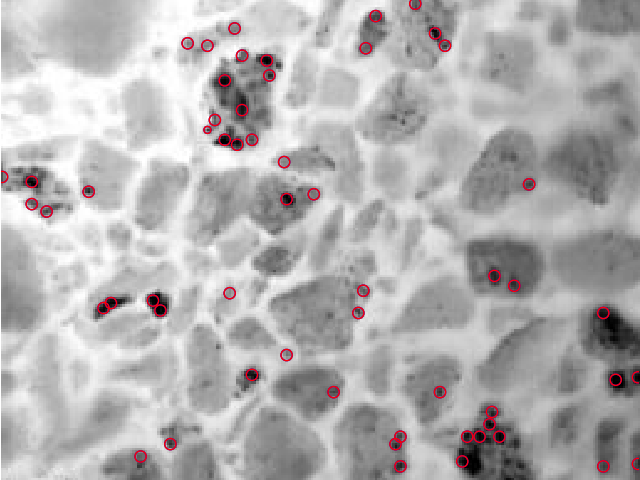
\includegraphics[width=0.8\textwidth]{blob_tracker_min_0}
        \caption{Obraz z~próbki 104\_E5R\_0}
    \end{subfigure}
    \hfill
    \begin{subfigure}[t]{0.45\textwidth}
        \centering
        \caption*{\scriptsize
            Minuta: 0, \\
            Liczba: wszystkich detali: 36, śledzonych detali: 29}
        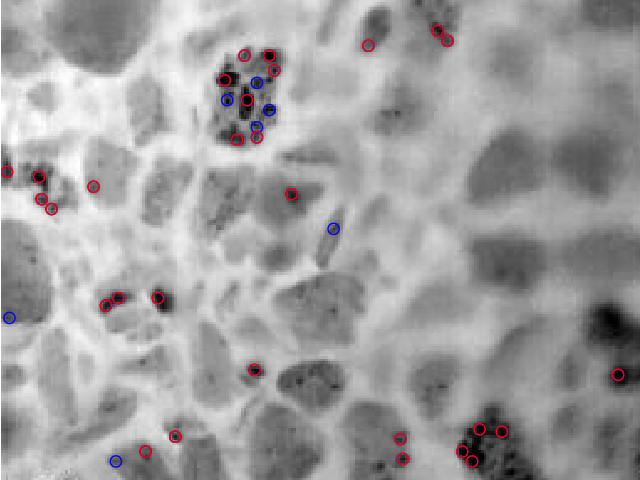
\includegraphics[width=0.8\textwidth]{blob_tracker_min_1}
        \caption{Obraz z~próbki 104\_E5R\_1}
    \end{subfigure}
    \hspace*{\fill}
    \vskip\baselineskip
    \hspace*{\fill}
    \begin{subfigure}[t]{0.45\textwidth}
        \centering
        \caption*{\scriptsize
            Minuta: 0, \\
            Liczba: wszystkich detali: 22, śledzonych detali: 16}
        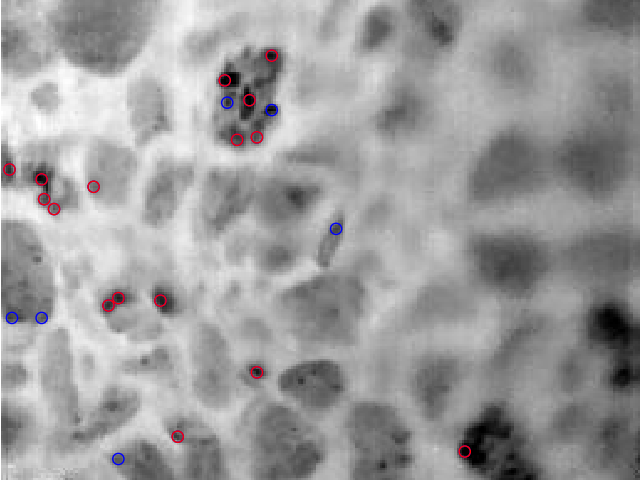
\includegraphics[width=0.8\textwidth]{blob_tracker_min_2}
        \caption{Obraz z~próbki 104\_E5R\_2}
    \end{subfigure}
    \hfill
    \begin{subfigure}[t]{0.45\textwidth}
        \centering
        \caption*{\scriptsize
            Minuta: 0, \\
            Liczba: wszystkich detali: 19, śledzonych detali: 13}
        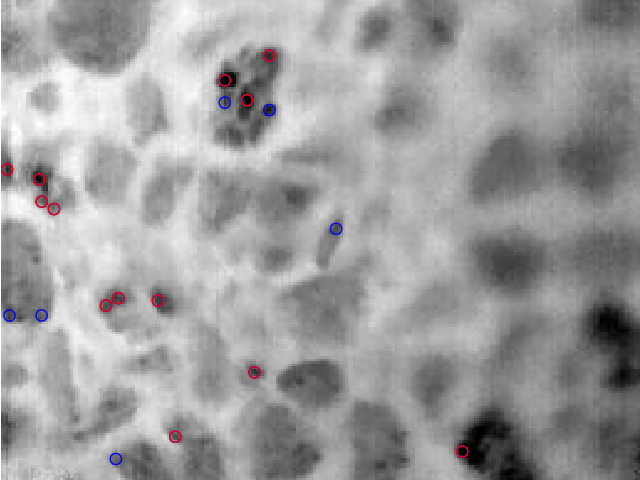
\includegraphics[width=0.8\textwidth]{blob_tracker_min_3}
        \caption{Obraz z~próbki 104\_E5R\_3}
    \end{subfigure}
    \hspace*{\fill}
    \vskip\baselineskip
    \hspace*{\fill}
    \begin{subfigure}[t]{0.45\textwidth}
        \centering
        \caption*{\scriptsize
            Minuta: 0, \\
            Liczba: wszystkich detali: 15, śledzonych detali: 11}
        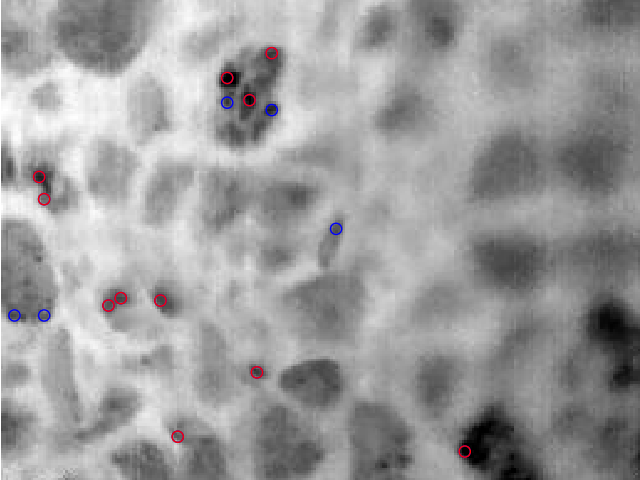
\includegraphics[width=0.8\textwidth]{blob_tracker_min_4}
        \caption{Obraz z~próbki 104\_E5R\_4}
    \end{subfigure}
    \hspace*{\fill}
    \begin{description} \footnotesize
        \centering
        \item[Kolor czerwony] detale śledzone od początku stygnięcia
        \item[Kolor niebieski] nowe wykryte detale
    \end{description}
    \caption{Zliczanie śledzonych detali w~próbce dwoma sposobami}
    \label{fig:blob_count}
\end{figure}

Metodę śledzenia plam i~ich zanikania przedstawiono na rysunku
\ref{fig:blob_remain}.~%
Pokazuje on położenie plam wykrytych w~kolejnych etapach stygnięcia.
Wykryte punkty zaznaczono na obrazie z~początku tego procesu.
Zmieniające się kolory obrazują detale wykryte w~kolejnych chwilach.
Pozawala to zaobserwować przemieszczanie się środków ciężkości i~promieni plam
podczas stygnięcia i zlewania się.
\begin{figure}[tb]
    \centering
    \caption*{\scriptsize Detekcja metodą laplasjanu funkcji Gaussa}
    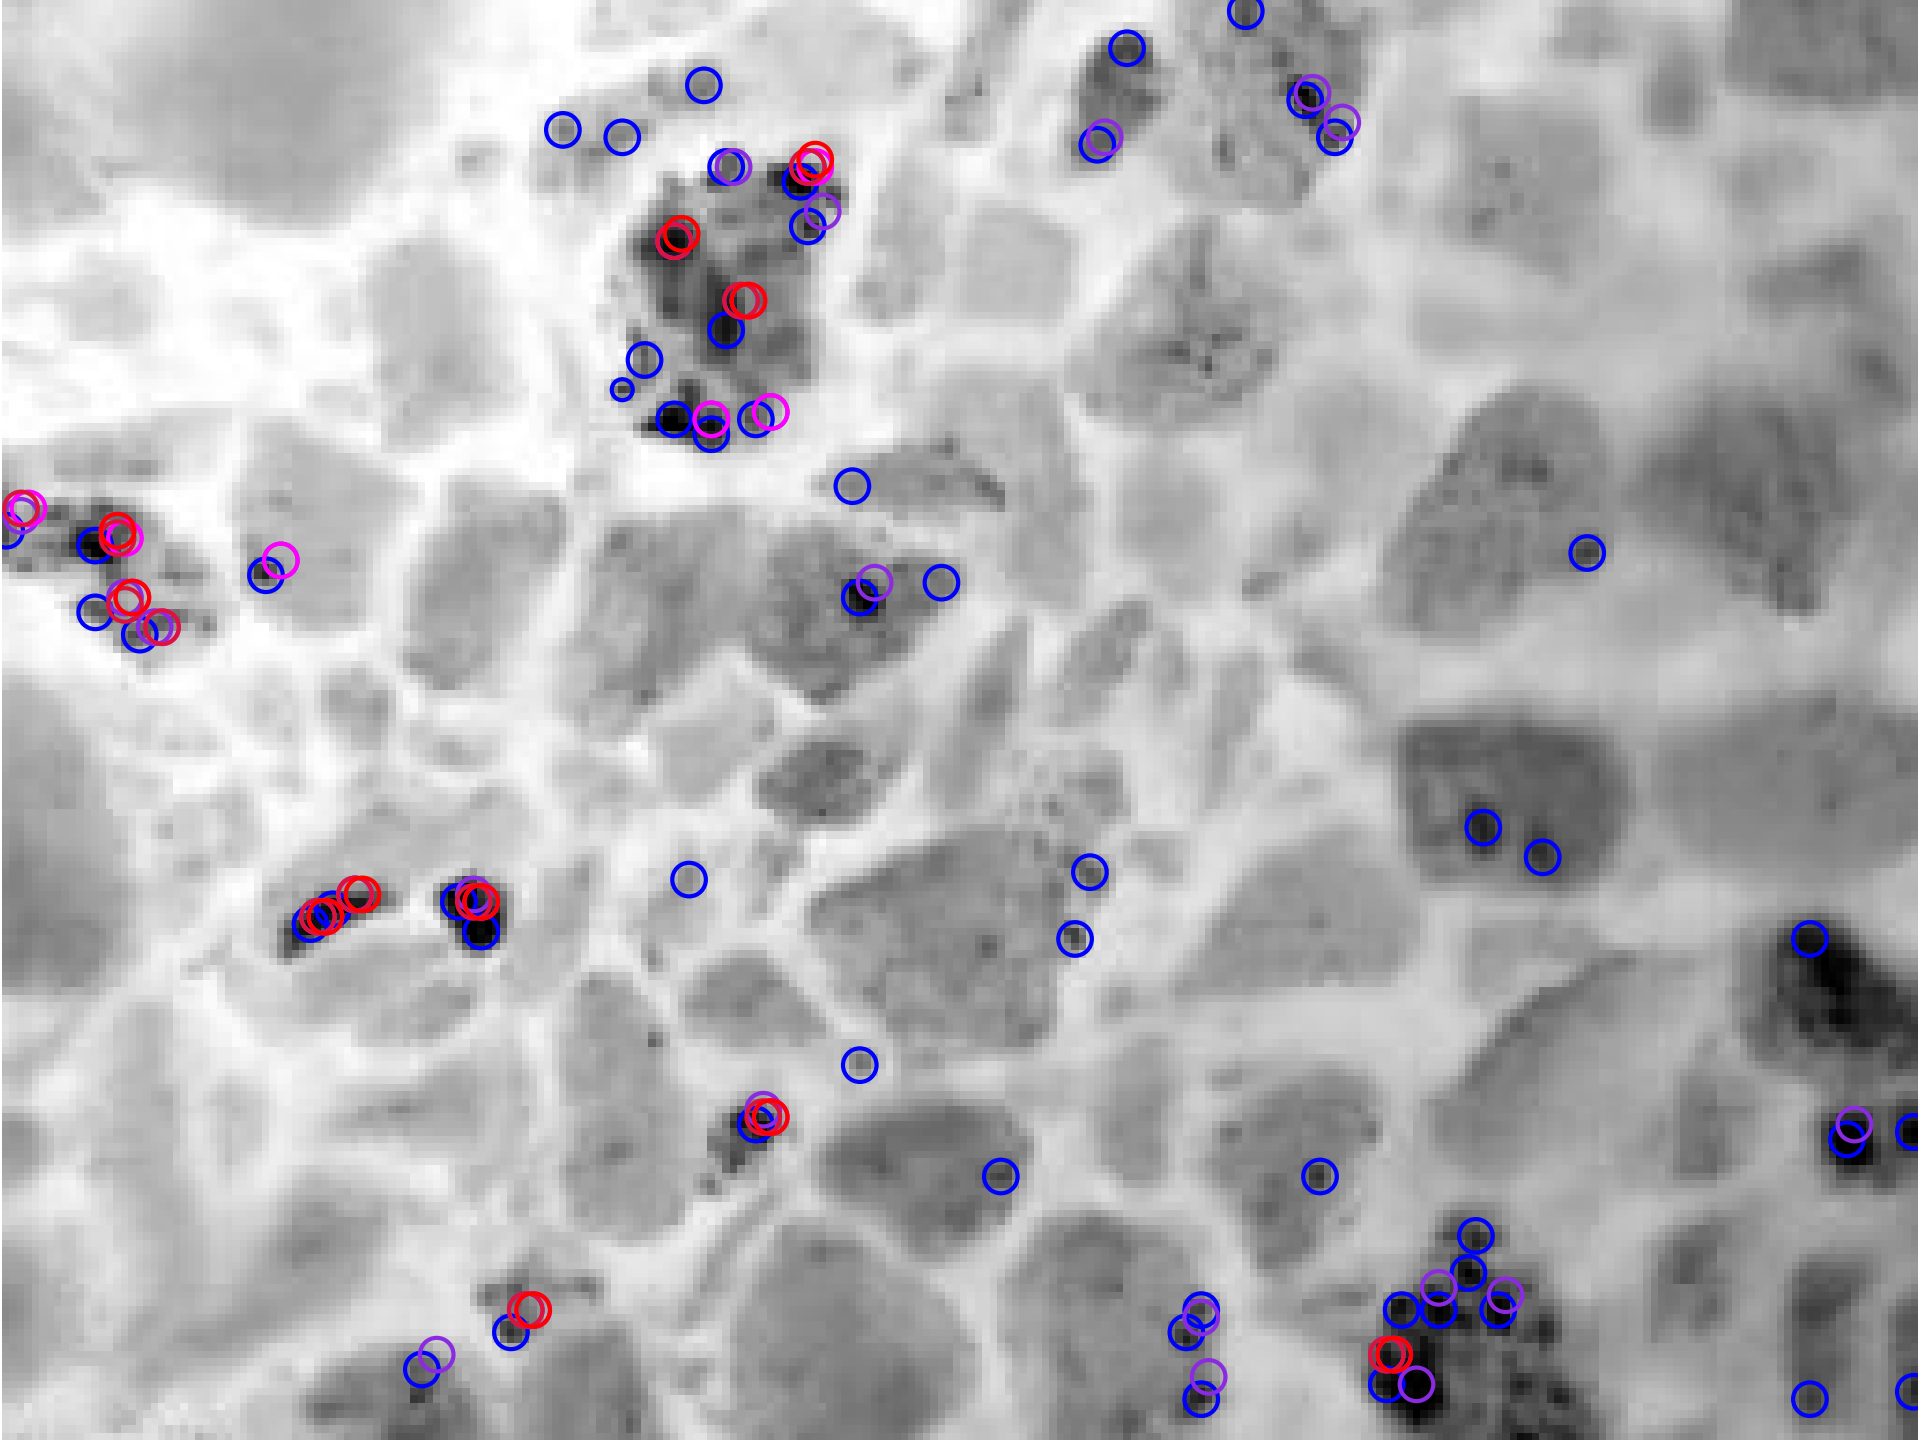
\includegraphics[width=0.5\textwidth]{blob_tracker}
    \vspace{0.3cm}
    \caption*{\scriptsize
        Kolorem niebieskim zaznaczono detale wykryte na początku stygnięcia.
        Wraz z~upływem czasu kolor oznaczenia detali przechodzi w~czerwień}
    \caption{Wykryte detale, śledzone od początku stygnięcia, zaznaczone na
        pierwszym obrazie w~serii pomiarowej}
    \label{fig:blob_remain}
\end{figure}
Działanie metody \ref{it:ratio_blob},~zliczającej stosunek śledzonych detali
do ich pierwotnej liczby zobrazowano w~tabeli \ref{tab:blob_ratio}.~%
Działanie zliczania przedstawiono dla każdej rozpatrywanej klasy ziaren.
\begin{table}[tb]
    \centering
    \begin{tabular}{c|c|c|c|c|c}
        \toprule
        Próbka    & Minuta 0 & Minuta 1 & Minuta 2 & Minuta 3 & Minuta 4 \\
        \midrule
        104\_E5R  & 1.0      & 0.52     & 0.29     & 0.23     & 0.20     \\
        107\_E6R  & 1.0      & 0.20     & 0.12     & 0.02     & 0.02     \\
        106\_E11R & 1.0      & 0.12     & 0.02     & 0.00     & 0.00     \\
        111\_E16R & 1.0      & 0.05     & 0.01     & 0.01     & 0.01     \\
        \bottomrule
    \end{tabular}
    \caption{Stosunek liczby detali śledzonych w~kolejnych etapach stygnięcia do
        ich liczby na początku pomiaru}
    \label{tab:blob_ratio}
\end{table}

\subsection{Wizualizacja zebranych cech i~ocena ich użyteczności}
\label{subsec:data_vis}
W~podsekcji \ref{subsec:blob_tracking}~przedstawiono opracowane algorytmy
śledzenia ilości detali w~rozpatrywanych obrazach stygnięcia ziaren rud miedzi.
Opracowane metody mają sens przy klasyfikacji, jeśli pozyskane cechy są
charakterystyczne dla rozpatrywanych klas.
Aby oszacować użyteczność pozyskanych cech należy przeprowadzić ich
wizualizację.
W~tym celu stworzono wykresy ilości wykrytych plam dla poszczególnych metod ich
zliczania.

Rysunek \ref{fig:blob_chart_all}~przedstawia wykres procesu zanikania plam dla
wariantu z~wykrywaniem wszystkich detali na każdym etapie stygnięcia.
\begin{figure}[tb]
    \centering
    \input{figures/blob_analysis_all}
    \caption{Liczba wykrytych detali na~każdym etapie stygnięcia, w~wariancie
        zliczającym wszystkie plamy}
    \label{fig:blob_chart_all}
\end{figure}
Wykreślone krzywe dla różnych klas materiałów przecinają się, na wykresach nie
widać uporządkowania, ani wyraźnych zależności.
Liczba charakterystycznych detali może być cechą ziaren rud miedzi, ze względu
na ich różną budowę, jednak w~analizowanym przypadku nie jest to cecha dająca
nadzieję na dobre wyniki klasyfikacji.
Powodem takiej sytuacji jest duża losowość tego typu danych.
Niezależnie od własności materiału, jego ułożenie podczas pomiaru jest
przypadkowe, co ma wpływ na bezwzględną liczbę zliczonych detali.
Na liczbę widocznych plam wpływa również sposób ustawienia ostrości kamery.
Po przyjrzeniu się wykresom można jednak domniemywać, że pewną cechą
charakterystyczną jest nachylenie krzywych.
Wskazuje to, że bardziej widoczne mogą być względne cechy czasowe, a~nie
bezwzględna liczba zliczonych detali.

Efekty drugiego sposób zliczania punktów przedstawiono na rysunku
\ref{fig:blob_chart_rem}.~%
\begin{figure}[tb]
    \centering
    \input{figures/blob_analysis_remaining}
    \caption{Liczba detali wykrytych na zdjęciach, w~wariancie zliczającym
        plamy śledzone od początku procesu stygnięcia}
    \label{fig:blob_chart_rem}
\end{figure}
W~tym przypadku zliczano jedynie detale obecne na obrazie od początku
stygnięcia.
Ten wariant śledzenia ilości plam daje dużo lepsze perspektywy na klasyfikację
ziaren.
Dla różnych typów próbek widoczne są charakterystyczne przebiegi krzywych.
Obserwacja dotycząca nachylenia krzywych staje się bardziej uzasadniona,
pochodne poszczególnych klas wydają się zbliżone.
Wyeliminowanie pojawiających się detali pomogło w~obserwacji procesu stygnięcia
i~zmniejszyło czynniki losowe.
Na podstawie analizy nagrań można domniemywać, że nowe ziarna pojawiały się
w~wyniku zaobserwowanych delikatnych ruchów materiału.
Te mogły wynikać z~drgań stanowiska pomiarowego, istotnym czynnikiem może być
także mała głębia ostrości obiektywu.
W~późniejszych etapach stygnięcia na obrazach pojawia się także coraz więcej
szumów, które mogą zostać wykryte przez algorytm.
Śledzenie detali, które znajdują się na obrazie od początku eliminuje ten
problem.

Wyniki ostatniej metody, polegającej na ustaleniu stosunku śledzonych detali
do ich pierwotnej liczby, został przedstawiona na rysunku
\ref{fig:blob_chart_ratio}.~%
\begin{figure}[tb]
    \centering
    \input{figures/blob_analysis_ratio}
    \caption{Stosunek śledzonych detali do ich liczby na początku procesu
        stygnięcia}
    \label{fig:blob_chart_ratio}
\end{figure}
Widoczne jest odseparowanie różnych klas rud miedzi, różne typy próbek
charakteryzują się odmiennymi postępami rozmycia detali w~czasie.
Śledzenie ilości detali w~stosunku względnym dało najlepsze rezultaty.
Nastąpiła także pewna normalizacja danych, która była trudna do realizacji przy
bezwzględnym zliczaniu wszystkich plam na obrazie.
Należy także zauważyć, że przedstawione krzywe przedstawione na rysunkach
\ref{fig:blob_chart_rem}~oraz \ref{fig:blob_chart_ratio}~mają kształt zbliżony
do krzywych eksponencjalnych.
Jest to obserwacja wskazująca, że pozyskane cechy dobrze oddają naturę procesu
stygnięcia.
Proces opadania temperatury ciał opisuje \emph{prawo stygnięcia Newtona}, które
ma postać równania różniczkowego, przedstawionego we wzorze
\ref{eq:newton_law_diff}~\cite{lienhard_heat}.
\begin{equation}
    \frac{dT \left( t \right)}{dt}=-k\left( T \left( t \right) -T_{R} \right)
    \label{eq:newton_law_diff}
\end{equation}%
\begin{samepage}
Oznaczenia we wzorze mają następujące znaczenia:
\begin{description}
    \item $ T \left( t \right) $ to funkcja temperatury ciała w~czasie,
    \item $ T_R $ to temperatura otocznia,
    \item $ k $ to współczynnik liczbowy, charakterystyczny dla danego ciała.
\end{description}
\end{samepage}
Rozwiązanie równania przedstawia wzór \ref{eq:newton_law},~jak widać ma ono
charakter eksponencjalny, do którego zbliżone są wykresy na rysunkach
\ref{fig:blob_chart_rem}~oraz \ref{fig:blob_chart_ratio}.
\begin{equation}
    T(t) - T_{R} = \Delta T (t) = \Delta T (0) \ e^ {-k t}
    \label{eq:newton_law}
\end{equation}

Analiza pozyskanych cech wskazuje, że istnieje możliwość ich wykorzystania
w~klasyfikacji rud miedzi.
Dalsza ocena wyników pracy będzie zależała od jakości działania sieci neuronowej
stworzonej do rozpoznawania przygotowanych danych.
